\begin{enumerate}

\item  The coordinates of point $\vec{P}$ dividing the line $AB$ in the ratio $m:n$ is given by 
\begin{align}
\vec{P} &= \frac{m\vec{B}+n\vec{A}}{m+n}  \label{vec/2/26/2.0.2}
\\
&=\frac{2\myvec{3\\4\\-5}+3\myvec{1\\-2\\3}}
{(2+3)}
\\
&=\myvec{{\frac{9}{5}} \\ {\frac{2}{5}} \\ {\frac{-1}{5}}}
\end{align}
which is verified in Fig.     \ref{vec/2/26/fig:Internally.}
\begin{figure}[!ht]
    \centering
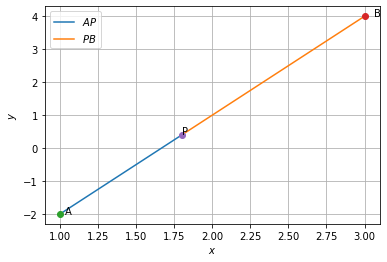
\includegraphics[width=\columnwidth]{solutions/su2021/2/26/internally.png}
    \caption{INTERNALLY}
    \label{vec/2/26/fig:Internally.}
\end{figure} 

\item  The coordinates of point $\vec{Q}$ dividing the line $AB$ in the ratio $m:n$ is given by 
\begin{align}
 \vec{Q} &= \frac{m\vec{B}-n\vec{A}}{m+n}  \label{vec/2/26/2.0.5}
 \\
&=\frac{2\myvec{3\\4\\-5}-3\myvec{1\\-2\\3}}
{(2-3)}
\\
&=\myvec{-3\\-14\\19}
\end{align}
%
which is verified in Fig.     \ref{vec/2/26/fig:EXTERNALLY.}


\begin{figure}[!ht]
    \centering
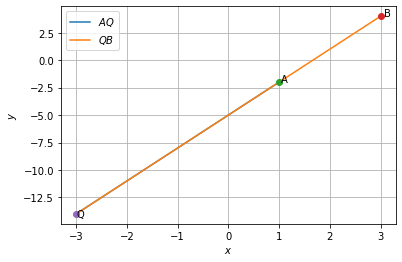
\includegraphics[width=\columnwidth]{solutions/su2021/2/26/externally.png}
    \caption{EXTERNALLY}
    \label{vec/2/26/fig:EXTERNALLY.}
\end{figure}  
\end{enumerate}
